给定平面上两条射线夹出的角, 仅凭直尺和圆规不一定能将其三等分. 
这是因为三等分角实际上涉及了开立方运算:
$$
\cos(3\theta)=-3\cos(\theta)+4\cos^3(\theta)
$$
其中 $3\theta$ 为已知角. 由于公理 (6) 可以实现开立方运算, 
由定理 3.2 知折纸三等分角是可以办到的. 
下面给出了一种实现方法 \cite{Hul}, 其证明是相似三角形的简单推导. 

\begin{figure}[h]
    \centering
    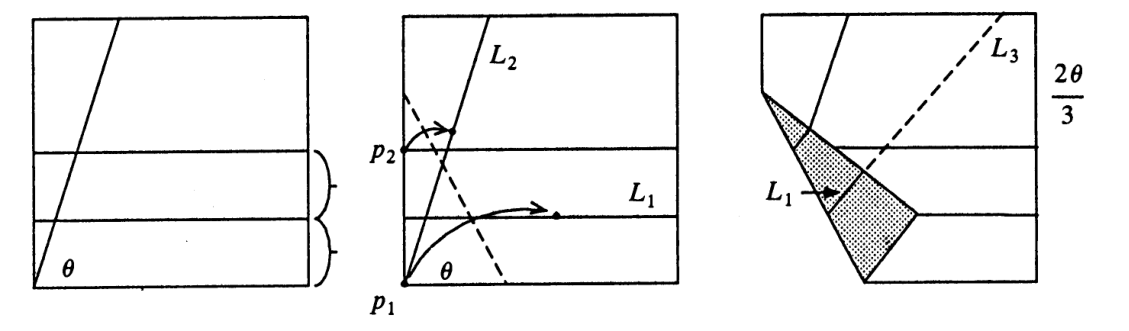
\includegraphics[scale=0.4]{trisect.png}
    \caption{三等分角}
\end{figure}